% Generated by code/ch01_duality.py -- do not edit by hand.
\definecolor{qocA}{rgb}{0.00,0.45,0.70}
\definecolor{qocB}{rgb}{0.90,0.60,0.00}
\definecolor{qocC}{rgb}{0.00,0.62,0.45}
\definecolor{qocD}{rgb}{0.80,0.40,0.00}
\definecolor{qocE}{rgb}{0.80,0.60,0.70}
\definecolor{qocF}{rgb}{0.35,0.70,0.90}
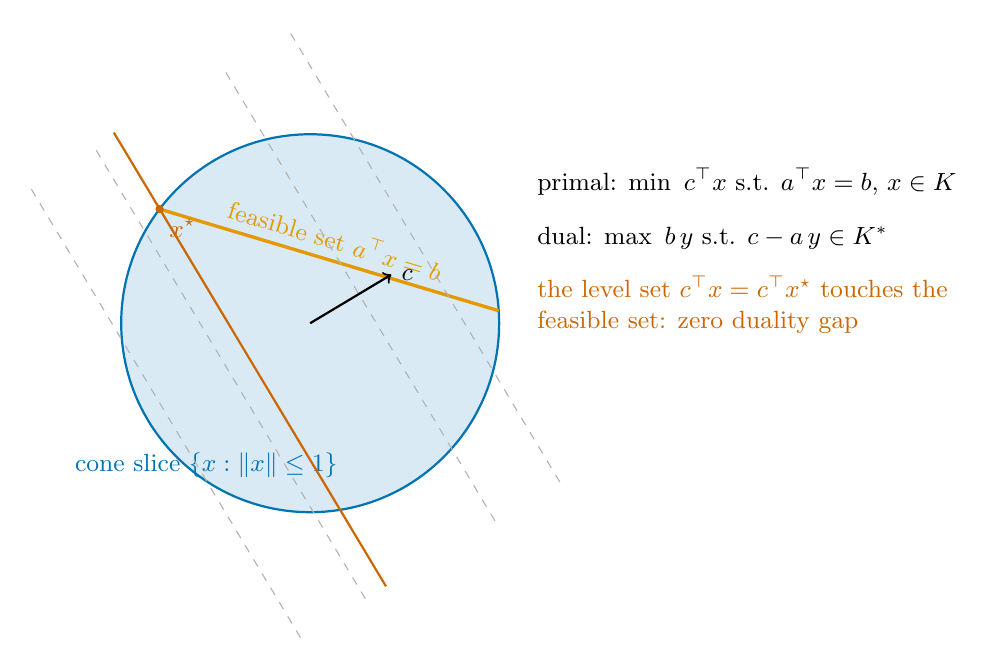
\begin{tikzpicture}[]

\begin{scope}[x=2.4cm,y=2.4cm]
\fill[qocA!15, draw=qocA, thick] (0,0) circle (1);
\node[text=qocA, font=\small] at (-0.55,-0.75) {cone slice $\{x: \|x\|\le 1\}$};
\draw[qocB, very thick] (0.998,0.066) -- (-0.797,0.604) node[pos=0.5, above, sloped, font=\small] {feasible set $a^\top x=b$};
\fill[qocD] (-0.797,0.604) circle (1.5pt) node[below right, font=\small] {$x^\star$};
\draw[gray!60, dashed] (-0.051,-1.664) -- (-1.492,0.737);
\draw[gray!60, dashed] (0.292,-1.458) -- (-1.149,0.943);
\draw[qocD, thick] (0.401,-1.392) -- (-1.039,1.009);
\draw[gray!60, dashed] (0.978,-1.046) -- (-0.463,1.355);
\draw[gray!60, dashed] (1.321,-0.840) -- (-0.120,1.561);
\draw[->, thick] (0,0) -- (0.429,0.257) node[right, font=\small] {$c$};
\node[font=\small, align=left, anchor=west] at (1.15,0.75) {primal: $\min\ c^\top x$ s.t. $a^\top x=b$, $x\in K$};
\node[font=\small, align=left, anchor=west] at (1.15,0.45) {dual: $\max\ b\,y$ s.t. $c-a\,y\in K^*$};
\node[font=\small, align=left, anchor=west, text=qocD] at (1.15,0.1) {the level set $c^\top x=c^\top x^\star$ touches the\\ feasible set: zero duality gap};
\end{scope}
\end{tikzpicture}
